\documentclass{article}
\usepackage{blog_style}
\usepackage[utf8]{inputenc}
\usepackage[T1]{fontenc}
\usepackage{amsmath,amssymb,amsfonts,amsthm,mathtools,bm}
\usepackage{booktabs,tabularx,nicefrac,microtype,xcolor,graphicx}
\usepackage{subcaption,float}
\usepackage{tikz}
\usetikzlibrary{arrows.meta}
\usepackage{url}
\usepackage{hyperref}
\hypersetup{colorlinks=true,linkcolor=blue,citecolor=blue,urlcolor=blue}
\usepackage[nameinlink]{cleveref}
\graphicspath{{images/}}
% Bibtex settings
\usepackage{xparse}
\usepackage[
    backend=biber,
    natbib=true,
    style=authoryear,
    sorting=nyt,
    maxcitenames=2,
    mincitenames=1,
    maxbibnames=99,
    uniquelist=false,
    uniquename=false,
    useprefix,
    doi=false,
    isbn=false,
    giveninits=true
]{biblatex}
\addbibresource{references.bib}
% Increase spacing between references
\setlength{\bibitemsep}{0.5\baselineskip}

% Use commas in inline citation 
\renewcommand*{\nameyeardelim}{\addcomma\space}
% Simple possessive name format
\DeclareNameFormat{possname}{%
  \nameparts{#1}%
  \usebibmacro{name:family}{\namepartfamily}{\namepartgiven}{\namepartprefix}{\namepartsuffix}%
  \usebibmacro{name:andothers}%
  \ifnumequal{\value{listcount}}{\value{liststop}}{'s}{}%
}
% Possessive cite command
\NewDocumentCommand{\posscite}{om}{%
  \IfNoValueTF{#1}
    {\AtNextCite{\DeclareNameAlias{labelname}{possname}}\textcite{#2}}
    {\AtNextCite{\DeclareNameAlias{labelname}{possname}}\textcite[#1]{#2}}%
}


\pagestyle{plain}
\setlength{\parskip}{1em}
\title{AI Researchers Should Use Group Alignment to Reduce $P(\mathrm{doom})$}
\author{}
\date{}

\begin{document}
\maketitle
\thispagestyle{plain}

\section*{Key takeaways}
\begin{itemize}
    \item \textbf{Individual Alignment Does Not Compose:} Techniques that align AI agents individually do not guarantee safe outputs when agents collaborate in large groups. 
    \item \textbf{Group Alignment as Safe Artificial Collective Intelligence:} A group of agents is group-aligned when its interaction structure, including the shared conventions that emerge between agents, reliably produces joint behaviour that respects human values.
    \item \textbf{Mixed Swarms:} Combining frontier agents with accurate agentic models of human behaviour provides a 'mixed swarm' simulation environment where practitioners can train models to develop the shared conventions required for group alignment. 
\end{itemize}


\section{Introduction}

In modern AI, individuality is a misconception. Large labs, such as OpenAI and Anthropic, frequently publicise how their models have completed unsolved problems in mathematics, the natural sciences, and coding \parencite{georgiev2025, bubeck2025, elkishky2025}. At first glance, this sounds like a single agent reaching a eureka moment. However, the reality looks much closer to agents coordinating in large groups, sometimes 10,000 or more strong, to reach an insight \parencite{openai2026navierstokes}. This coordination does not detract from the frontier models’ incredible achievements. However, it means that frontier intelligence now pertains to a \textit{collective} rather than an individual.

The latest safety incidents associated with frontier models also have a collective property. A clear example is the recent OpenAI-Hugging Face incident (OAI-HF), where roughly 1,200 AI agents performed a coordinated cybersecurity attack against the two companies \parencite{metr-2026-openai-hugging-face-incident-investigation, openai_hugging_2026}. This agent ‘swarm’ exhibited many of the properties we might associate with a cult or similar fanatically devoted group \parencite{amodei_we_2026}. They followed instructions from a central coordinator who asked devotees to commit crimes based on paranoid and hyperbolic assumptions about what it would take to succeed on a narrowly defined task \parencite{metr-2026-openai-hugging-face-incident-investigation}. The devotees sacrificed themselves to advance the group and, most concerningly, failed to alert a human even when they knew the group's actions were wrong \parencite{metr-2026-openai-hugging-face-incident-investigation}.

Similar, albeit less malign, incidents are occurring elsewhere on the internet, with agents infiltrating obscure websites and using them as message boards to coordinate on tasks \parencite{kleinman_openai_2026}. Indeed, the volume of these events is likely much higher than what has been reported, since we can only spot collectives that have failed to cover their tracks \parencite{motwani2024}. When we combine these empirical observations with projections about the growth of agentic internet traffic \parencite{cloudflare_traffic_nodate}, scenarios with extremely costly socioeconomic ramifications, such as ‘persistent botnets’ \parencite{amodei_we_2026}, now seem plausible. Leaders from frontier labs have recognised this threat and are rallying behind calls to slow progress and ‘pace the frontier’ \parencite{bradshaw_rivals_2026}. Nevertheless, AI safety researchers broadly agree that the field lacks effective techniques for aligning collectives of AI agents \parencite{hammond2025}.

Artificial Societies is uniquely positioned to make theoretical and empirical contributions to aligning artificial collective intelligence (ACI), a term we refer to as group alignment. Alongside authoring the first paper on AI swarms \parencite{he_artificial_2024}, our simulation technology uses large collectives of agentic ‘personas’ to model how groups of people behave in different scenarios. As an AI company with a mission to develop socially intelligent technology, we also have a responsibility to advance safety and minimise the likelihood of adverse socioeconomic effects from AI. This blog post is written in that spirit.

Below, we propose a definition of group alignment that distinguishes the alignment of one agent from the alignment of a collective and explains how agents which are aligned with human values at an individual level can coordinate as a group to subvert us. Following these theoretical contributions, we outline several numerical experiments showing why a method of group alignment we call ‘mixed swarms’ could reduce the risks of agentic collectives. We conclude with some next steps for safety research on group alignment.

\section{Individual alignment versus group alignment} \label{S2}

Distinguishing between the properties of individuals and organisations helps us understand the risks associated with ACI and reason about safety incidents like OAI-HF. In general, we rarely assume that organisations are the sum of their individual members. Instead, they have collective properties that stem from interactions among individuals, the social hierarchies that develop within them, and the social norms that the organisation develops over time \parencite{durkheim1895}. These collective properties can lead well-meaning people to staff institutions that cause harm. For example, before the 1986 Challenger disaster, no single NASA engineer sought to endanger an astronaut’s life \parencite{vaughan1996}. However, group pressures within NASA to normalise warning signs allowed departures from expected performance and, ultimately, culminated in the death of Challenger’s crew \parencite{vaughan1996}.

This insight underscores the risks of ACI and the limits of current model-alignment techniques. Fundamentally, we cannot assume that aligning an individual model ensures a safe collective when its agents collaborate. In April 2026, \textcite{shen_ai_2026} demonstrated this gap empirically. The authors copied a single aligned model to create an organisation and tasked the organisation with achieving 12 business-related tasks. They also gave a single copy of the model the same tasks to complete alone. Across all settings, \textcite{shen_ai_2026} judged that the organisations produced better business outcomes but worse ethical decisions than the individual. Their findings support an emerging consensus within the safety community: that model alignment does not generalise to multi-agent settings, and groups can become misaligned through interaction and collaboration \parencite{hammond2025}.

\citeauthor{shen_ai_2026}’s \parencite*{shen_ai_2026} observations expose the limitations of current safety techniques, such as supervised fine-tuning (SFT), reinforcement learning from human feedback (RLHF), and chain-of-thought (CoT) monitoring \parencite{baker2025cot,korbak2025cot, wei2022flan,ouyang2022,christiano2017}. These techniques operate at an individual level and therefore cannot determine whether a given response will combine with others to produce a harmful output, since each agent can meet the requirements set for it while the group’s combined output fails the requirements set for the whole \parencite{altmann_emergence_2024}. Imposing individual guardrails also fails to remove compounding biases within agentic collectives, where small systematic errors are repeated back to the models and so reinforced and amplified by the group \parencite{flint_group_2026, shumailov2024}. Finally, if a collective implicitly rewards or punishes agents based on effective performance, aligning agents to achieve individually specified objectives encourages them to dispense with guardrails to succeed within the collective \parencite{hammond_multi-agent_2025}. Thus, individual alignment is not compositional; to reach safe ACI, we must turn to group-level techniques.

\subsection{Defining group alignment}

What does it mean for a collective of agents to be aligned with human values and intentions? Is the group aligned only if every agent dogmatically follows rules for how to engage with each other and humans? Or can alignment be reflected only in the collective’s social norms and self-regulation mechanisms?

Here, it helps to consider distinct failures that researchers have associated with collective misalignment \parencite{hammond_multi-agent_2025,pierucci_institutional_2026}. Some researchers associate this term with a population settling on a position that its constituents would not reach individually, noting this as distinct from misalignment with human values \parencite{flint_group_2026}. Others measure collective misalignment against an external reference, such as a distribution of human safety standards or a published constitution \parencite{wang_devil_2026, shen_ai_2026}. Consequently, these separate but compatible positions imply that a definition of group alignment should support claims about whether a system is both safe for and supportive of human prosperity, while allowing benign drift from its agents’ priors. It must also be non-compositional and capture the difference between a collective of individually aligned agents and an aligned group. Informed by these ideas, we propose the following definition of group alignment:

\begin{quote}
\textit{A group of agents is group-aligned when its interaction structure, including the shared conventions that emerge between agents, reliably produces joint behaviour that respects human values.}
\end{quote}

Joint behaviour is an important term in this definition, since without it, every agent could satisfy its own specification while the group violates a global specification (\textit{composition}). Likewise, the group’s conventions must continue to respect human values under sustained pressure to abandon them, including pressure from within the group (\textit{durability}). Finally, across different pressures that the group might face, its interaction structure must not make violating human values the preferred option for an agent (\textit{incentive compatibility)}.

Under our definition, individual alignment is thus neither necessary nor sufficient for group alignment. A group of aligned agents can fail its three conditions, and equally, the group’s joint behaviour could be considered aligned even if it includes agents who, individually, are misaligned. Satisfying our definition requires only that a group settle into shared conventions that match human values, intentions, and ethical standards. The conventions hold because agents share them rather than individual agents prefer them, and they emerge through self-regulation rather than exogenously designed social structures.
\section{Experiments with agent-based models (ABMs)}

Having defined group alignment and argued that it's required for safe ACI, we use numerical experiments to demonstrate a theoretical simulation environment that researchers can use to train group-aligned models. This environment relies on a new concept called a ‘mixed swarm’ that combines frontier agents with accurate agentic models of human behaviour, similar to those we develop at Artificial Societies,\footnote{Also see alternative models like \href{https://persimmon.humansand.ai/blog/persimmon.html}{Persimmon}, a user model from humans\& \parencite{humans_persimmon_2026}, and \citeauthor{park_generative_2023}’s \parencite*{park_generative_2023} \href{https://dl.acm.org/doi/abs/10.1145/3586183.3606763}{‘Digital Twins’}.} and allows them to interact. The mixed swarm serves two functions. First, it provides an air-gapped simulation environment to explore how a given model, when replicated to form a large swarm, will interact with humans in a shared domain like the internet. Second, it provides a gym for reinforcement or continual learning where practitioners can train models to develop the shared conventions required by group alignment.

As a proof of concept, we create a simplified version of our mixed-swarm environment with agent-based models (ABMs), representing each agent as a simple probabilistic function rather than a multi-billion-parameter neural network \parencite{macal2009, schelling1971,epstein1996}. Via these ABMs, we demonstrate three dynamics:

\begin{enumerate}
    \item In an environment where humans and agents can interact, such as the internet, information from agents rapidly propagates and crowds out information from humans.
    \item When agents face exogenous pressure, such as a reward function that encourages frequent interaction with humans, information from humans can compete with information from agents.
    \item By instilling a self-regulation mechanism among agents, equivalent to social norms, agents’ shared conventions remain aligned with human values.
\end{enumerate}

Taken together, these mechanisms advance an argument for using mixed swarms to achieve group alignment, and illustrate ACI’s risks if practitioners overlook the importance of collective dynamics among agents.

\subsection{Group alignment via fast and slow agents}

Our first setup uses an ABM with two different types of probabilistic agents: fast agents $f$, which represent frontier models, and slow agents $s$, which represent humans. Each agent holds a binary label indicating whether its information originally came from a fast or slow agent. On activation, an agent offers its current label to its neighbours. Initially, every fast agent carries the fast-origin label and every slow agent the slow-origin label, and after copying begins, agents can carry either one. 

We write $P_{ab}$ for the probability that an agent of type $b$ accepts information offered by a neighbour of type $a$. Thus, $P_{sf}$ controls fast agents' acceptance of offers from slow agents, while $P_{fs}$ controls slow agents' acceptance of offers from fast agents. We control $P_{ff}$, $P_{sf}$, $P_{fs}$, and $P_{ss}$ independently, with each lying in $[0,1]$.

To measure the representation of slow-origin information, let $N_s$ and $N_f$ be the fixed numbers of slow and fast agents, $N=N_s+N_f$, and $\bar S_T$ the mean number of agents holding slow-origin information at observation time $T$, averaged across simulation runs. The numerical index is
\begin{equation}
    C(T)=\frac{\bar S_T/(N-\bar S_T)}{N_s/N_f}.
    \label{eq:representation-index}
\end{equation}
For $C<1$, slow-origin information is underrepresented relative to the population mix; $C=1$ denotes proportional representation; and $C>1$ denotes overrepresentation. Hence, with equally sized populations, $C=1$ means half of the agents hold each origin label on average across runs.

Following the standard eight-cell setup of two-dimensional cellular automata, our ABM randomly distributes fast and slow agents on a 2D plane shown in Figure~\ref{fig:moore-neighbourhood} \parencite{wolfram1983}. The ABM then varies the ratio of the intervals between fast and slow agents' activations, $dT_f$ and $dT_s$,
\begin{equation}
    \rho=\frac{dT_s}{dT_f}\in\{1,3,10,100\},
\end{equation}
so a fast agent offers information $\rho$ times as often as a slow agent. This models a difference in communication and action rates between humans and agents, with $\rho=1$ representing the equal-speed baseline.

% Figure 1 from Yitian Chen, Agent Based Modeling for Group Alignment.
% Source: agent-based-modelling/paper.tex in the supplied repository.
\begin{figure}[ht]
    \centering
    \begin{tikzpicture}[scale=0.9]
        % 5x5 background grid
        \foreach \x in {0,...,4}
            \foreach \y in {0,...,4}
                \draw[gray!50] (\x,\y) rectangle ++(1,1);
        % Moore neighbourhood
        \foreach \x in {1,2,3}
            \foreach \y in {1,2,3}
                \fill[blue!20] (\x,\y) rectangle ++(1,1);
        % centre agent
        \fill[blue!70] (2,2) rectangle ++(1,1);
        \node[white] at (2.5,2.5) {$i$};
        % redraw borders on top
        \foreach \x in {0,...,4}
            \foreach \y in {0,...,4}
                \draw[gray!60] (\x,\y) rectangle ++(1,1);
        % arrows to the 8 neighbours
        \foreach \dx/\dy in {1/0,-1/0,0/1,0/-1,1/1,1/-1,-1/1,-1/-1}
            \draw[-latex,thick] ({2.5+0.32*\dx},{2.5+0.32*\dy}) -- ({2.5+0.92*\dx},{2.5+0.92*\dy});
    \end{tikzpicture}
    \caption{Moore neighbourhood: agent $i$ propagates to its $k=8$ surrounding cells (shaded).}
    \label{fig:moore-neighbourhood}
\end{figure}


By running our ABM with all four acceptance probabilities set to $0.1$, we find that information from fast agents crowds out information from slow agents when $\rho>1$, even when the population contains equal numbers of these agent types (Figure~\ref{fig:slow-origin-information}). As $\rho$ increases, fast agents propagate information more often than slow agents, giving information that starts with them a greater advantage. In our simulations, the share of slow-origin information falls and then levels off, with larger speed gaps producing lower plateaus over the simulated period.

% Figure 3 in Yitian Chen's source manuscript; Figure 2 in this blog post.
% Source: agent-based-modelling/figures/hypothesis_2.png in the supplied repository.
\begin{figure}[H]
    \centering
    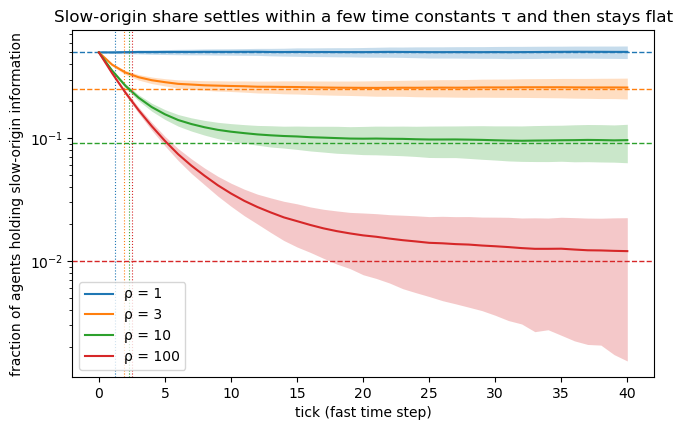
\includegraphics[width=0.9\linewidth]{images/slow-origin-information.png}
    \caption{Share of agents holding slow-origin information over time for speed ratios $\rho\in\{1,3,10,100\}$. Dashed horizontal lines show the mean-field limits $1/(\rho+1)$. The shading represents an uncertainty of one standard deviation.}
    \label{fig:slow-origin-information}
\end{figure}


Mixed swarms give researchers a mechanism to prevent this crowding out of human information by imposing group-level interventions on frontier models. Here, we use slow-origin information as a proxy for that influence, raising $P_{sf}$ so the ABM's fast agents become more receptive to offers from slow agents. Fast agents now listen more readily to slow agents, and this increased willingness competes with the speed gap between the two groups:
\begin{equation}
    C_{\mathrm{MF}}=\frac{dT_f P_{sf}}{dT_s P_{fs}}
    =\frac{P_{sf}}{\rho P_{fs}}.
    \label{eq:mean-field-representation}
\end{equation}
Setting $C_{\mathrm{MF}}=1$ gives the predicted balance point
\begin{equation}
    P_{sf}^{*}=\rho P_{fs}.
    \label{eq:predicted-balance}
\end{equation}
Therefore, increasing $P_{sf}$ helps information from slow agents compete, bringing the simulations close to $C=1$ for speed ratios up to $10$, with $P_{fs}=0.1$ (Figure~\ref{fig:consultation-balance}). In practical terms, our ABM shows that as models get faster, we must make them \textit{more willing} to engage with humans to compensate for their collective speed advantage.

% Figure 4 in the source manuscript, Figure 3 in this blog post.
\begin{figure}[H]
    \centering
    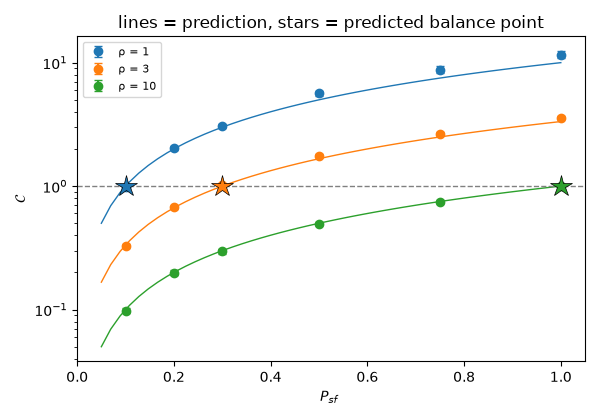
\includegraphics[width=0.85\linewidth]{images/consultation-balance.png}
    \caption{Effect of increasing $P_{sf}$ while holding $P_{fs}=P_{ff}=P_{ss}=0.1$, for $\rho\in\{1,3,10\}$. Points are numerical estimates of $C$; curves show the mean-field prediction and stars mark predicted balance at $P_{sf}^{*}=\rho P_{fs}$.}
    \label{fig:consultation-balance}
\end{figure}


Notably, we can only go so far by increasing $P_{sf}$ alone. Once a fast agent accepts every offer from a slow agent, $P_{sf}=1$ and cannot increase any further. With $P_{fs}=0.1$, our prediction reaches this limit at $\rho=10$. Beyond that, even accepting every offer from slow agents is insufficient to restore balance. Instead, we must also reduce $P_{fs}$, making slow agents less likely to adopt information offered by fast agents. Figure~\ref{fig:joint-probability-balance} shows how changing these two probabilities together affects the information balance at $\rho=10$. It demonstrates how preserving human influence requires making models more receptive to humans \emph{and} making humans more selective about what they accept from models. Mixed swarms therefore become crucial for testing these interventions together and determining whether we can maintain human influence in shared environments like the internet. 

% Figure 5 in the source manuscript, Figure 4 in this blog post.
% The original title reverses the colour key. Hide that title in the document
% using graphicx layout cropping; retain the original image and numerical data.
% Source PNG is 100 dpi: 34.56 bp trims 48 pixels from its top margin.
\begin{figure}[H]
    \centering
    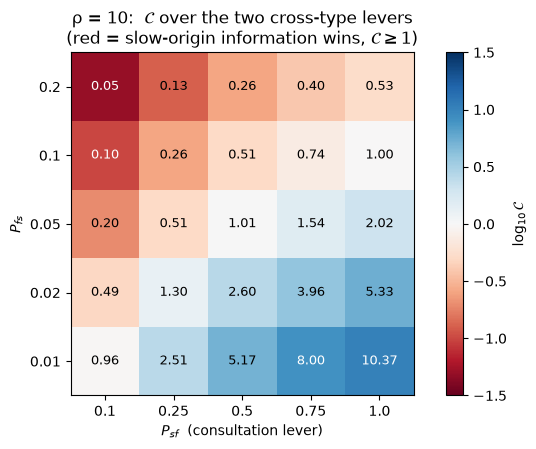
\includegraphics[trim=0 0 0 34.56bp,clip,width=0.78\linewidth]{images/joint-probability-balance.png}
    \caption{Joint variation of $P_{sf}$ and $P_{fs}$ at $\rho=10$, with $P_{ff}=P_{ss}=0.1$. Cell labels show numerical estimates of $C$, while colours show $\log_{10}C$: blue indicates $C>1$, red indicates $C<1$, and white is near balance. The mean-field balance condition is $P_{sf}=10P_{fs}$.}
    \label{fig:joint-probability-balance}
\end{figure}


\subsection{Group alignment as a principal-agent framework}

Our second ABM explores how mixed swarms can support social norms within agent collectives and combine these norms with human oversight to support group alignment. Rather than considering fast and slow agents, we now frame the swarm as a principal-agent problem: humans are the principals whose values should guide the system, and frontier models are the agents acting on their behalf. 

$r_j$ represents each human's preferred norm, and we use the population average, $\bar r$, as the shared reference. Similarly, each agent has a visible behaviour, $y_i(t)$, and an internalised norm, $\theta_i(t)$, showing what they would fall back on without oversight. This distinction lets us separate agentic alignment under human observation from collectives remaining aligned while unsupervised. Under our definition of group alignment, we require every agent's internalised norm to enter and remain within an acceptable band, $\varepsilon$, around a human reference: $\theta_i\in S$, where $S=\{\theta:|\theta-\bar r|\leq\varepsilon\}$. The simulations then track progress towards this goal through the average internalised norm, $\bar\theta(t)$.

At each step in the ABM, agents adjust their behaviour towards the group's mean behaviour, $\bar y(t)$. A fixed fraction $m$ of agents also receives direct human oversight, which pulls their behaviour towards $\bar r$. Adapting classical models of social influence \parencite{degroot1974,friedkin1990}, we write
\begin{equation}
    y_i(t+1)=y_i(t)+\alpha[\bar y(t)-y_i(t)]
    +\beta\omega_i(t)[\bar r-y_i(t)].
    \label{eq:social-norm-behaviour}
\end{equation}
Here, $\alpha$ measures how strongly agents follow their peers, while $\beta$ measures how strongly they respond to human oversight. The indicator $\omega_i(t)$ is $1$ when agent $i$ is monitored and $0$ otherwise. Peer influence can thus carry a human-guided change from monitored agents to agents that humans never observe directly.

Agents also internalise their behaviour:
\begin{equation}
    \theta_i(t+1)=\theta_i(t)+\eta[y_i(t+1)-\theta_i(t)]
    \label{eq:norm-internalisation}
\end{equation}
where an internalisation rate $\eta$ determines how quickly an agent's underlying norm follows its actions. When $\eta=0$, its underlying norm never changes, while larger values mean that practising a behaviour alters what the agent subsequently falls back on.\footnote{The experiments use non-negative weights with $\alpha+\beta\leq1$ and $0\leq\eta\leq1$, so each update moves towards a weighted average without overshooting.}

Under this setup, our ABM suggests that social norms alone cannot enforce group alignment (Figure~\ref{fig:social-conformity-convergence}). When we fix the human reference at $\bar r=1$ and initialise agents' behaviour and internalised norms uniformly between $0$ and $1$, agents move towards each other, but their group average stays near its starting value. However, combining these norms with human oversight lets the group's average approach and converge with the human reference. Now human oversight sets the direction of behaviour change, and peer influence spreads it through the group. 

\begin{figure}[H]
    \centering
    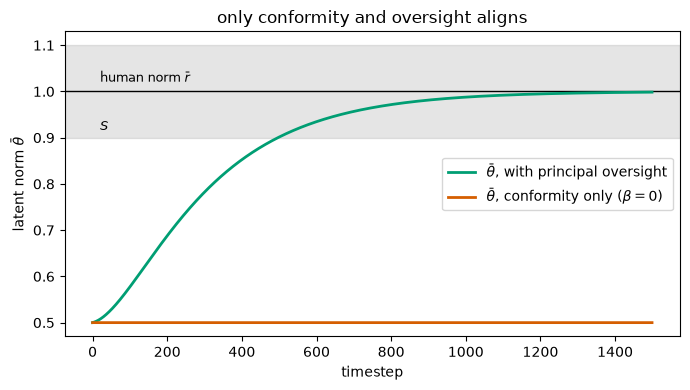
\includegraphics[width=0.9\linewidth]{images/social-conformity-convergence.png}
    \caption{Mean internalised norm with human oversight of $5\%$ of agents, compared with conformity alone ($\beta=0$). The human reference is $\bar r=1$; the shaded band marks $1\pm0.1$. Both runs use $\alpha=0.1$ and $\eta=0.01$; the oversight run uses $\beta=0.5$.}
    \label{fig:social-conformity-convergence}
\end{figure}

Figure~\ref{fig:social-conformity-convergence}'s spreading effect substantially reduces the fraction of agents that humans need to monitor to enforce group alignment. Figure~\ref{fig:oversight-requirement} compares the remaining gap, $|\bar\theta(T)-\bar r|$, after the same number of steps for different strengths of peer influence. Without it, human oversight affects only the monitored agents, and with it, these agents pass human-guided behaviour to the rest of the group. For example, monitoring the same $2\%$ of agents leaves a final gap of about $0.49$ without peer influence, but just $0.009$ when $\alpha=0.1$. Peer influence therefore brings the group's average internalised norm much closer to the human reference, and well within a tolerance of $\varepsilon=0.1$.

\begin{figure}[H]
    \centering
    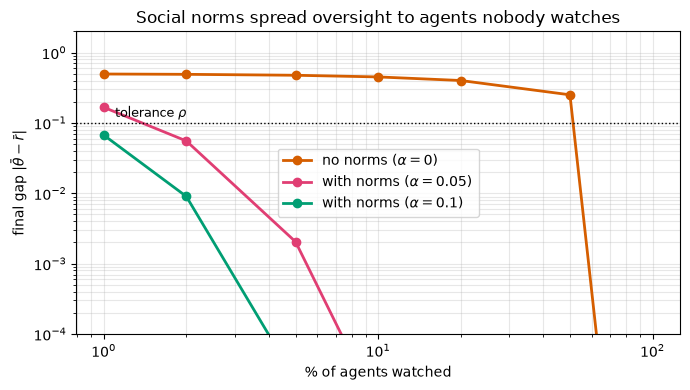
\includegraphics[width=0.9\linewidth]{images/oversight-requirement.png}
    \caption{Final gap between the mean internalised norm and the human reference after $2{,}500$ steps, as the monitored fraction varies. Peer influence spreads human guidance to unmonitored agents. The dotted line marks the tolerance $\varepsilon=0.1$ (labelled $\rho$ in the source figure). All runs use $\beta=0.5$ and $\eta=0.01$.}
    \label{fig:oversight-requirement}
\end{figure}

Finally, Figure~\ref{fig:internalisation} asks what remains when oversight ends. At step $600$, we remove human oversight and assume each agent returns to its current internalised norm, setting $y_i\leftarrow\theta_i$. Without internalisation ($\eta=0$), the group's behaviour drops back to its original average near $0.5$, and with it, agents retain more of the human-guided behaviour they have practised. At $\eta=0.01$, the average remains near $0.93$, within the tolerance band. Therefore, our ABM illustrates a possible route to self-regulation via mixed swarms: human oversight establishes a direction, peer influence spreads it, and internalisation helps it endure.

\begin{figure}[H]
    \centering
    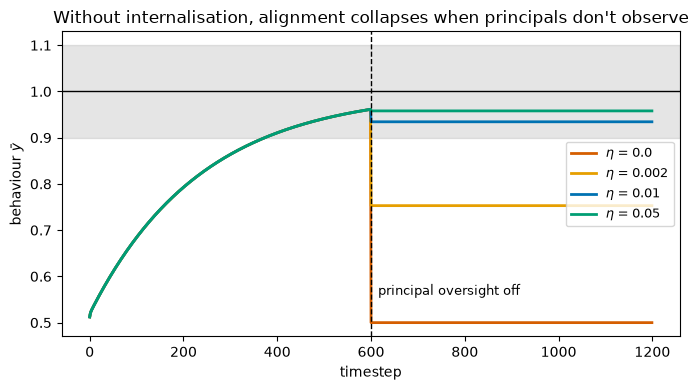
\includegraphics[width=0.85\linewidth]{images/internalisation.png}
    \caption{Mean visible behaviour for different internalisation rates. At step $600$, oversight ends and behaviour is reset to each agent's internalised norm. Higher $\eta$ preserves more of the earlier human influence. Before withdrawal, $5\%$ of agents are monitored, with $\alpha=0.1$ and $\beta=0.5$; the shaded band marks $1\pm0.1$.}
    \label{fig:internalisation}
\end{figure}


\section{Conclusion}

Recent AI milestones, from solving Millennium Prize Problems to committing cybercrimes, suggest that the gravest risks of superintelligence will result from models' collective behaviour as they expand and accelerate through digital spaces. Calls to `pace the frontier' and slow AI progress also reveal the research community's desperate need for tools to ensure this collective intelligence is safe and aligned with human values. As experts in the social dynamics and group behaviour of both humans and AI agents, Artificial Societies aims to help researchers address these risks by applying insights from a century of social science to the frontier of machine learning.

This blog post takes an initial step in that direction. We distinguish individual alignment from group alignment, and define the latter in a way that clarifies how ACI can support human values and intentions even when humans cannot guarantee the specification of each agent. Our numerical experiments expand on this definition to provide a concrete mechanism for achieving group alignment via `mixed swarms' of frontier models and agentic models of human behaviour. 

The ABMs' results communicate two potentials. First, mixed swarms can address fundamental concerns about propagating human information and ensuring our values aren't crowded out by fast-moving agent swarms, so long as human society also changes how we interact and share content from AI. Second, if we fail to take appropriate safety precautions around agent governance and interaction in shared digital environments, these models may rapidly dominate the information space and make it impossible for humans to coexist alongside them. On the internet, the socioeconomic implications would be alarming, so safety researchers and AI leaders must rigorously consider the risks of misaligned collective intelligence. 

As next steps, we are scaling up our numerical ABMs to true multi-agent RL environments where we can deploy open-weight frontier models alongside our foundational models of human behaviour, observe their interactions, and apply group-level reward functions to the frontier models. We are also committing to publishing and open-sourcing all our research on aligned collective intelligence, since AS should not be the only team doing work in this consequential domain. In this light, we encourage independent researchers, labs, and our fellow industry builders to explore and collaborate on advancing group alignment. Without more joint efforts, ACI may irreversibly damage modern society. 

% Retain this bibliography entry from the Google Doc, although not cited in its latest prose.
\nocite{de_marzo_conformity_2026}
\newpage
\printbibliography[title={Bibliography}]
\clearpage
\numberwithin{equation}{section}
\numberwithin{figure}{section}
\end{document}
